% Page: Hypothesis tests
% sources/stat2004/chapters/inf-04-hypothesis-tests.qmd
% Z = (Xbar - mu_0)/(sigma/sqrt(n)) is standard normal under H_0 when sigma
% is known. The two-sided level 0.05 critical value on that page is 1.960.
% The p-value is twice the tail beyond the observed |z|. The right panel is
% one alternative, Z ~ N(delta, 1) with delta = (mu - mu_0)/(sigma/sqrt(n)) = 2.
\documentclass[border=6pt]{standalone}
\usepackage[T1]{fontenc}
\usepackage{lmodern}
\usepackage{amsmath,amssymb}
\usepackage{tikz}
\usetikzlibrary{calc}
\usepackage{pgfplots}
\usepgfplotslibrary{fillbetween}
\pgfplotsset{compat=1.18}
\definecolor{ink}{HTML}{1F2430}
\definecolor{statblue}{HTML}{174A7E}
\definecolor{accent}{HTML}{9C4A32}
\definecolor{accentfill}{HTML}{F4E4DC}
\definecolor{bluefill}{HTML}{D7E5F0}
\definecolor{grey}{HTML}{5E6A75}
\pgfplotsset{
  stat/.style={
    scale only axis,
    axis lines=left,
    axis line style={ink, line width=0.6pt},
    tick style={ink, line width=0.45pt},
    tick label style={font=\small, text=ink},
    label style={font=\small, text=ink},
    title style={font=\small, text=ink, align=center},
    unbounded coords=jump,
    scaled ticks=false,
    set layers,
  },
}
\begin{document}
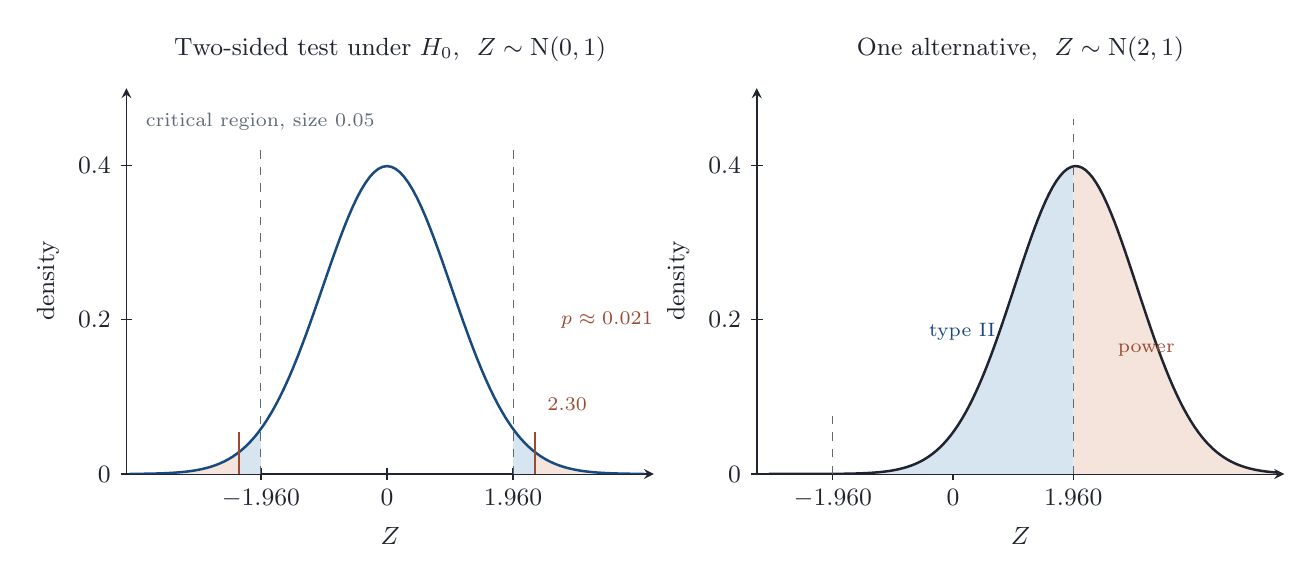
\begin{tikzpicture}
\begin{axis}[
  stat, name=h0, width=6.7cm, height=4.9cm,
  xmin=-4.05, xmax=4.15, ymin=0, ymax=0.50,
  xtick={-1.960,0,1.960},
  xticklabels={$-1.960$,$0$,$1.960$},
  ytick={0,0.2,0.4},
  xlabel={$Z$},
  ylabel={density},
  title={Two-sided test under $H_0$, \ $Z\sim\operatorname{N}(0,1)$},
]
  \addplot[name path=n0, draw=none, domain=-4:4, samples=121] {exp(-x^2/2)/sqrt(2*pi)};
  \addplot[name path=z0, draw=none, domain=-4:4, samples=2] {0};
  \addplot[bluefill] fill between[of=n0 and z0, soft clip={domain=-4:-1.960}];
  \addplot[bluefill] fill between[of=n0 and z0, soft clip={domain=1.960:4}];
  \addplot[accentfill] fill between[of=n0 and z0, soft clip={domain=-4:-2.30}];
  \addplot[accentfill] fill between[of=n0 and z0, soft clip={domain=2.30:4}];
  \addplot[statblue, line width=0.9pt, domain=-4:4, samples=121] {exp(-x^2/2)/sqrt(2*pi)};
  \draw[grey, dashed, thin] (axis cs:-1.960,0) -- (axis cs:-1.960,0.42);
  \draw[grey, dashed, thin] (axis cs:1.960,0) -- (axis cs:1.960,0.42);
  \draw[accent, thin] (axis cs:2.30,0) -- (axis cs:2.30,0.055);
  \draw[accent, thin] (axis cs:-2.30,0) -- (axis cs:-2.30,0.055);
  \node[font=\scriptsize, accent, anchor=south west] at (axis cs:2.34,0.07) {$2.30$};
  \node[font=\scriptsize, accent, anchor=west] at (axis cs:2.55,0.20)
    {$p\approx 0.021$};
  \node[font=\scriptsize, grey, anchor=north west, align=left] at (axis cs:-3.9,0.48)
    {critical region, size $0.05$};
\end{axis}

\begin{axis}[
  stat, width=6.7cm, height=4.9cm,
  at={($(h0.outer north east)+(1.15,0)$)}, anchor=outer north west,
  xmin=-3.2, xmax=5.4, ymin=0, ymax=0.50,
  xtick={-1.960,0,1.960},
  xticklabels={$-1.960$,$0$,$1.960$},
  ytick={0,0.2,0.4},
  xlabel={$Z$},
  ylabel={density},
  title={One alternative, \ $Z\sim\operatorname{N}(2,1)$},
]
  \addplot[name path=n1, draw=none, domain=-3:5.3, samples=141] {exp(-(x-2)^2/2)/sqrt(2*pi)};
  \addplot[name path=z1, draw=none, domain=-3:5.3, samples=2] {0};
  \addplot[bluefill] fill between[of=n1 and z1, soft clip={domain=-1.960:1.960}];
  \addplot[accentfill] fill between[of=n1 and z1, soft clip={domain=1.960:5.3}];
  \addplot[ink, line width=0.9pt, domain=-3:5.3, samples=141] {exp(-(x-2)^2/2)/sqrt(2*pi)};
  \draw[grey, dashed, thin] (axis cs:-1.960,0) -- (axis cs:-1.960,0.08);
  \draw[grey, dashed, thin] (axis cs:1.960,0) -- (axis cs:1.960,0.46);
  \node[font=\scriptsize, statblue, anchor=south] at (axis cs:0.15,0.16) {type II};
  \node[font=\scriptsize, accent, anchor=south] at (axis cs:3.15,0.14) {power};
\end{axis}
\end{tikzpicture}
\end{document}
